% !TEX encoding = UTF-8
% !TEX TS-program = xelatex
\documentclass[12pt, a4paper]{article}

% --- CÁC GÓI CHO XELATEX ---
\usepackage{polyglossia}
\setdefaultlanguage{vietnamese}

\usepackage{fontspec}
\setmainfont{Times New Roman}

% --- CÁC GÓI ĐỊNH DẠNG ---
\usepackage[a4paper, margin=1in]{geometry}
\usepackage{graphicx}
\graphicspath{{./images/}}
\usepackage{amsmath}
\usepackage[colorlinks=true, linkcolor=blue, urlcolor=blue, citecolor=red]{hyperref}

% --- THÔNG TIN DỰ ÁN ---
\title{
\vspace{-1.5cm}

\includegraphics[width=0.3\textwidth]{logo.png} \\[1em]
Fichain: Nền Tảng Blockchain Layer 1 \\
Kiến Tạo Tương Lai Ngân Hàng Số
}

\author{%
  Phan Đình Minh Hiếu \\
  Phạm Bảo Hân \\
  Trần Ngọc Hải \\
  Nguyễn Di Nguy \\
  Hà Kiệt Hùng
}
\date{\today}

\begin{document}

\maketitle
\thispagestyle{empty}
\newpage

\tableofcontents % Tạo mục lục tự động
\newpage

% --- NẠP NỘI DUNG TỪ CÁC TỆP CON ---
\section{Tóm tắt dự án}
Fichain là nền tảng blockchain Layer 1 hiệu suất cao, an toàn và tuân thủ, được thiết kế chuyên biệt cho các nghiệp vụ lõi của ngành tài chính - ngân hàng. Dự án ra đời nhằm giải quyết các thách thức của ngành ngân hàng khi ứng dụng công nghệ blockchain, bao gồm các rào cản từ hệ thống truyền thống, chi phí tích hợp cao, và những lo ngại về bảo mật, tuân thủ quy định.

Giải pháp của Fichain là cung cấp một nền tảng "sẵn sàng sử dụng" (turnkey), giúp các ngân hàng và tổ chức tài chính nhanh chóng phát triển và triển khai các sản phẩm tài chính số. Nền tảng nổi bật với cơ chế đồng thuận \textbf{PoSA (Proof of Staked Authority)}\cite{BinanceAcademy_PoSA} độc đáo, khả năng tương thích hoàn toàn với \textbf{EVM (Ethereum Virtual Machine)}\cite{wood2014ethereum}, và năng lực xử lý hàng nghìn giao dịch mỗi giây (TPS).

Điểm khác biệt chiến lược của dự án là việc \textbf{sử dụng Việt Nam Đồng(VNĐ) làm đơn vị tiền tệ gốc (native coin)} được bảo chứng, giúp loại bỏ hoàn toàn rủi ro biến động giá, đơn giản hóa giao dịch và phù hợp tuyệt đối với môi trường pháp lý và nghiệp vụ ngân hàng. Fichain hướng đến mục tiêu trở thành hạ tầng nền tảng cho kỷ nguyên số của ngành ngân hàng Việt Nam, với công nghệ được làm chủ hoàn toàn bởi đội ngũ kỹ sư trong nước.

\section{Mô tả chi tiết}

\subsection{Bối cảnh và vấn đề}
Ngành ngân hàng toàn cầu đang đối mặt với áp lực hiện đại hóa để nâng cao năng lực cạnh tranh và đáp ứng kỳ vọng của khách hàng trong kỷ nguyên số. Tuy nhiên, quá trình này gặp phải nhiều rào cản lớn:
\begin{itemize}
  \item \textbf{Hệ thống truyền thống:} Các hệ thống core banking truyền thống thường cứng nhắc, khó mở rộng và tốn kém để bảo trì, gây khó khăn khi tích hợp công nghệ mới.\cite{haralayya2021core}
  \item \textbf{Chi phí và độ phức tạp:} Việc áp dụng các công nghệ mới như blockchain đòi hỏi chi phí đầu tư lớn và chuyên môn kỹ thuật sâu, đặc biệt là việc tự xây dựng một nền tảng blockchain riêng.\cite{koteska2017blockchain}
  \item \textbf{Bảo mật và tuân thủ:} Các blockchain công cộng phổ biến (permissionless) như Ethereum thường có chi phí giao dịch biến động và không đáp ứng được các yêu cầu khắt khe về tính riêng tư\cite{peng2021privacy}, định danh (KYC/AML) và tuân thủ quy định của Ngân hàng Nhà nước.\cite{Vietnamese2023ND13,Vietnamese2022Luat14,Vietnamese2023ND19,Vietnamese2023TT09}
  \item \textbf{Xu hướng toàn cầu:} Sự ra đời của các sáng kiến blockchain quốc gia như EBSI (European Blockchain Services Infrastructure)\cite{ebsi2020} của Liên minh châu Âu và BSN (Blockchain-based Service Network)\cite{bsn2020} của Trung Quốc cho thấy các cường quốc đang chủ động phát triển hạ tầng blockchain riêng để bảo đảm chủ quyền dữ liệu, thúc đẩy chuyển đổi số và hỗ trợ các dịch vụ công nghệ số hiện đại. Điều này đặt ra yêu cầu cấp thiết để Việt Nam cũng cần có một nền tảng blockchain riêng nhằm không bị tụt hậu trong cuộc đua công nghệ toàn cầu.
\end{itemize}

\subsection{Giải pháp đề xuất: Nền tảng Fichain}
Fichain là một nền tảng blockchain Layer 1 được thiết kế chuyên biệt cho lĩnh vực tài chính - ngân hàng, nhằm giải quyết các rào cản trong quá trình chuyển đổi số:

\begin{itemize}
  \item \textbf{Tối ưu cho hệ thống tài chính:} Fichain cung cấp bộ công cụ và SDK dễ tích hợp với hệ thống core banking hiện có, hỗ trợ các giao diện API linh hoạt, giúp ngân hàng từng bước hiện đại hóa mà không cần thay đổi toàn bộ kiến trúc hiện tại.
  
  \item \textbf{Tiết kiệm chi phí và đơn giản hóa triển khai:} Fichain cung cấp một hạ tầng blockchain hoàn chỉnh dưới dạng dịch vụ (Blockchain-as-a-Service), giúp ngân hàng tránh được chi phí đầu tư ban đầu lớn và gánh nặng vận hành, đồng thời được hỗ trợ kỹ thuật chuyên sâu.
  
  \item \textbf{Tuân thủ pháp lý và bảo mật dữ liệu:} Fichain hỗ trợ cơ chế định danh, phân quyền truy cập (permissioned blockchain) và lưu trữ dữ liệu theo chuẩn trong nước, bảo đảm tuân thủ các quy định về bảo mật, KYC/AML và các nghị định liên quan của Ngân hàng Nhà nước.
  
  \item \textbf{Phù hợp với xu hướng quốc tế:} Tương tự như EBSI của châu Âu hay BSN của Trung Quốc, Fichain hướng đến mục tiêu xây dựng một hạ tầng blockchain quốc gia cho Việt Nam, nhằm bảo vệ chủ quyền dữ liệu, nâng cao năng lực số hóa ngành ngân hàng, và hỗ trợ phát triển các dịch vụ công nghệ tài chính hiện đại.
\end{itemize}

Với Fichain, các tổ chức tài chính tại Việt Nam không chỉ có cơ hội nâng cấp hạ tầng theo tiêu chuẩn quốc tế, mà còn góp phần chủ động tham gia vào hệ sinh thái số của quốc gia trong tương lai.

\subsection{Công nghệ cốt lõi}
Nền tảng Fichain được xây dựng từ gốc để đáp ứng các yêu cầu đặc thù của ngành tài chính.
\begin{itemize}
    \item \textbf{Native Coin là Việt Nam Đồng (VNĐ):} Một trong những khác biệt lớn nhất của Fichain là việc sử dụng đồng Việt Nam làm đơn vị tiền tệ gốc của mạng lưới. Về bản chất, đây là một dạng stablecoin được bảo chứng 1:1 với tiền pháp định (fiat). Điều này mang lại các lợi ích then chốt:
    \begin{itemize}
        \item Loại bỏ hoàn toàn biến động giá trị, vốn là rủi ro lớn nhất khi dùng các crypto-asset thông thường trong nghiệp vụ ngân hàng.
        \item Đơn giản hóa việc hạch toán, báo cáo và đối soát cho các tổ chức tài chính.
        \item Giúp người dùng cuối dễ dàng hiểu và tiếp cận, vì mọi giao dịch đều được định giá bằng đơn vị tiền tệ quen thuộc.
    \end{itemize}
    
    \item \textbf{Cơ chế đồng thuận PoSA (Proof of Staked Authority):} Đây là cơ chế lai kết hợp giữa PoA và PoS. Các validator (nút xác thực giao dịch) không chỉ phải được định danh và có uy tín (Authority - ví dụ: các ngân hàng trong liên minh) mà còn phải ký quỹ một lượng tài sản lớn (Stake). Mô hình này đảm bảo hiệu suất cao, bảo mật cấp doanh nghiệp và khả năng phân quyền có kiểm soát.

    \item \textbf{Tương thích EVM (Ethereum Virtual Machine):} Hỗ trợ đầy đủ EVM cho phép các nhà phát triển dễ dàng triển khai các hợp đồng thông minh (smart contract) viết bằng Solidity và các ứng dụng phi tập trung (DApps) từ hệ sinh thái Ethereum rộng lớn.
    
    \item \textbf{Mô hình mạng linh hoạt:} Fichain có thể được triển khai dưới dạng mạng riêng tư (private) cho một tổ chức, hoặc mạng liên minh (consortium) cho nhiều đối tác, đảm bảo tuân thủ các quy định về dữ liệu và bảo mật.
\end{itemize}

\subsection{Kiến trúc hệ thống}
Kiến trúc của Fichain được chia thành năm lớp chính, mỗi lớp đảm nhiệm một vai trò cụ thể trong hệ thống. Sơ đồ tổng quan được thể hiện trong Hình~\ref{fig:architecture}.

\begin{figure}[h!]
    \centering
    % The image architecture.png should be placed in the specified path.
    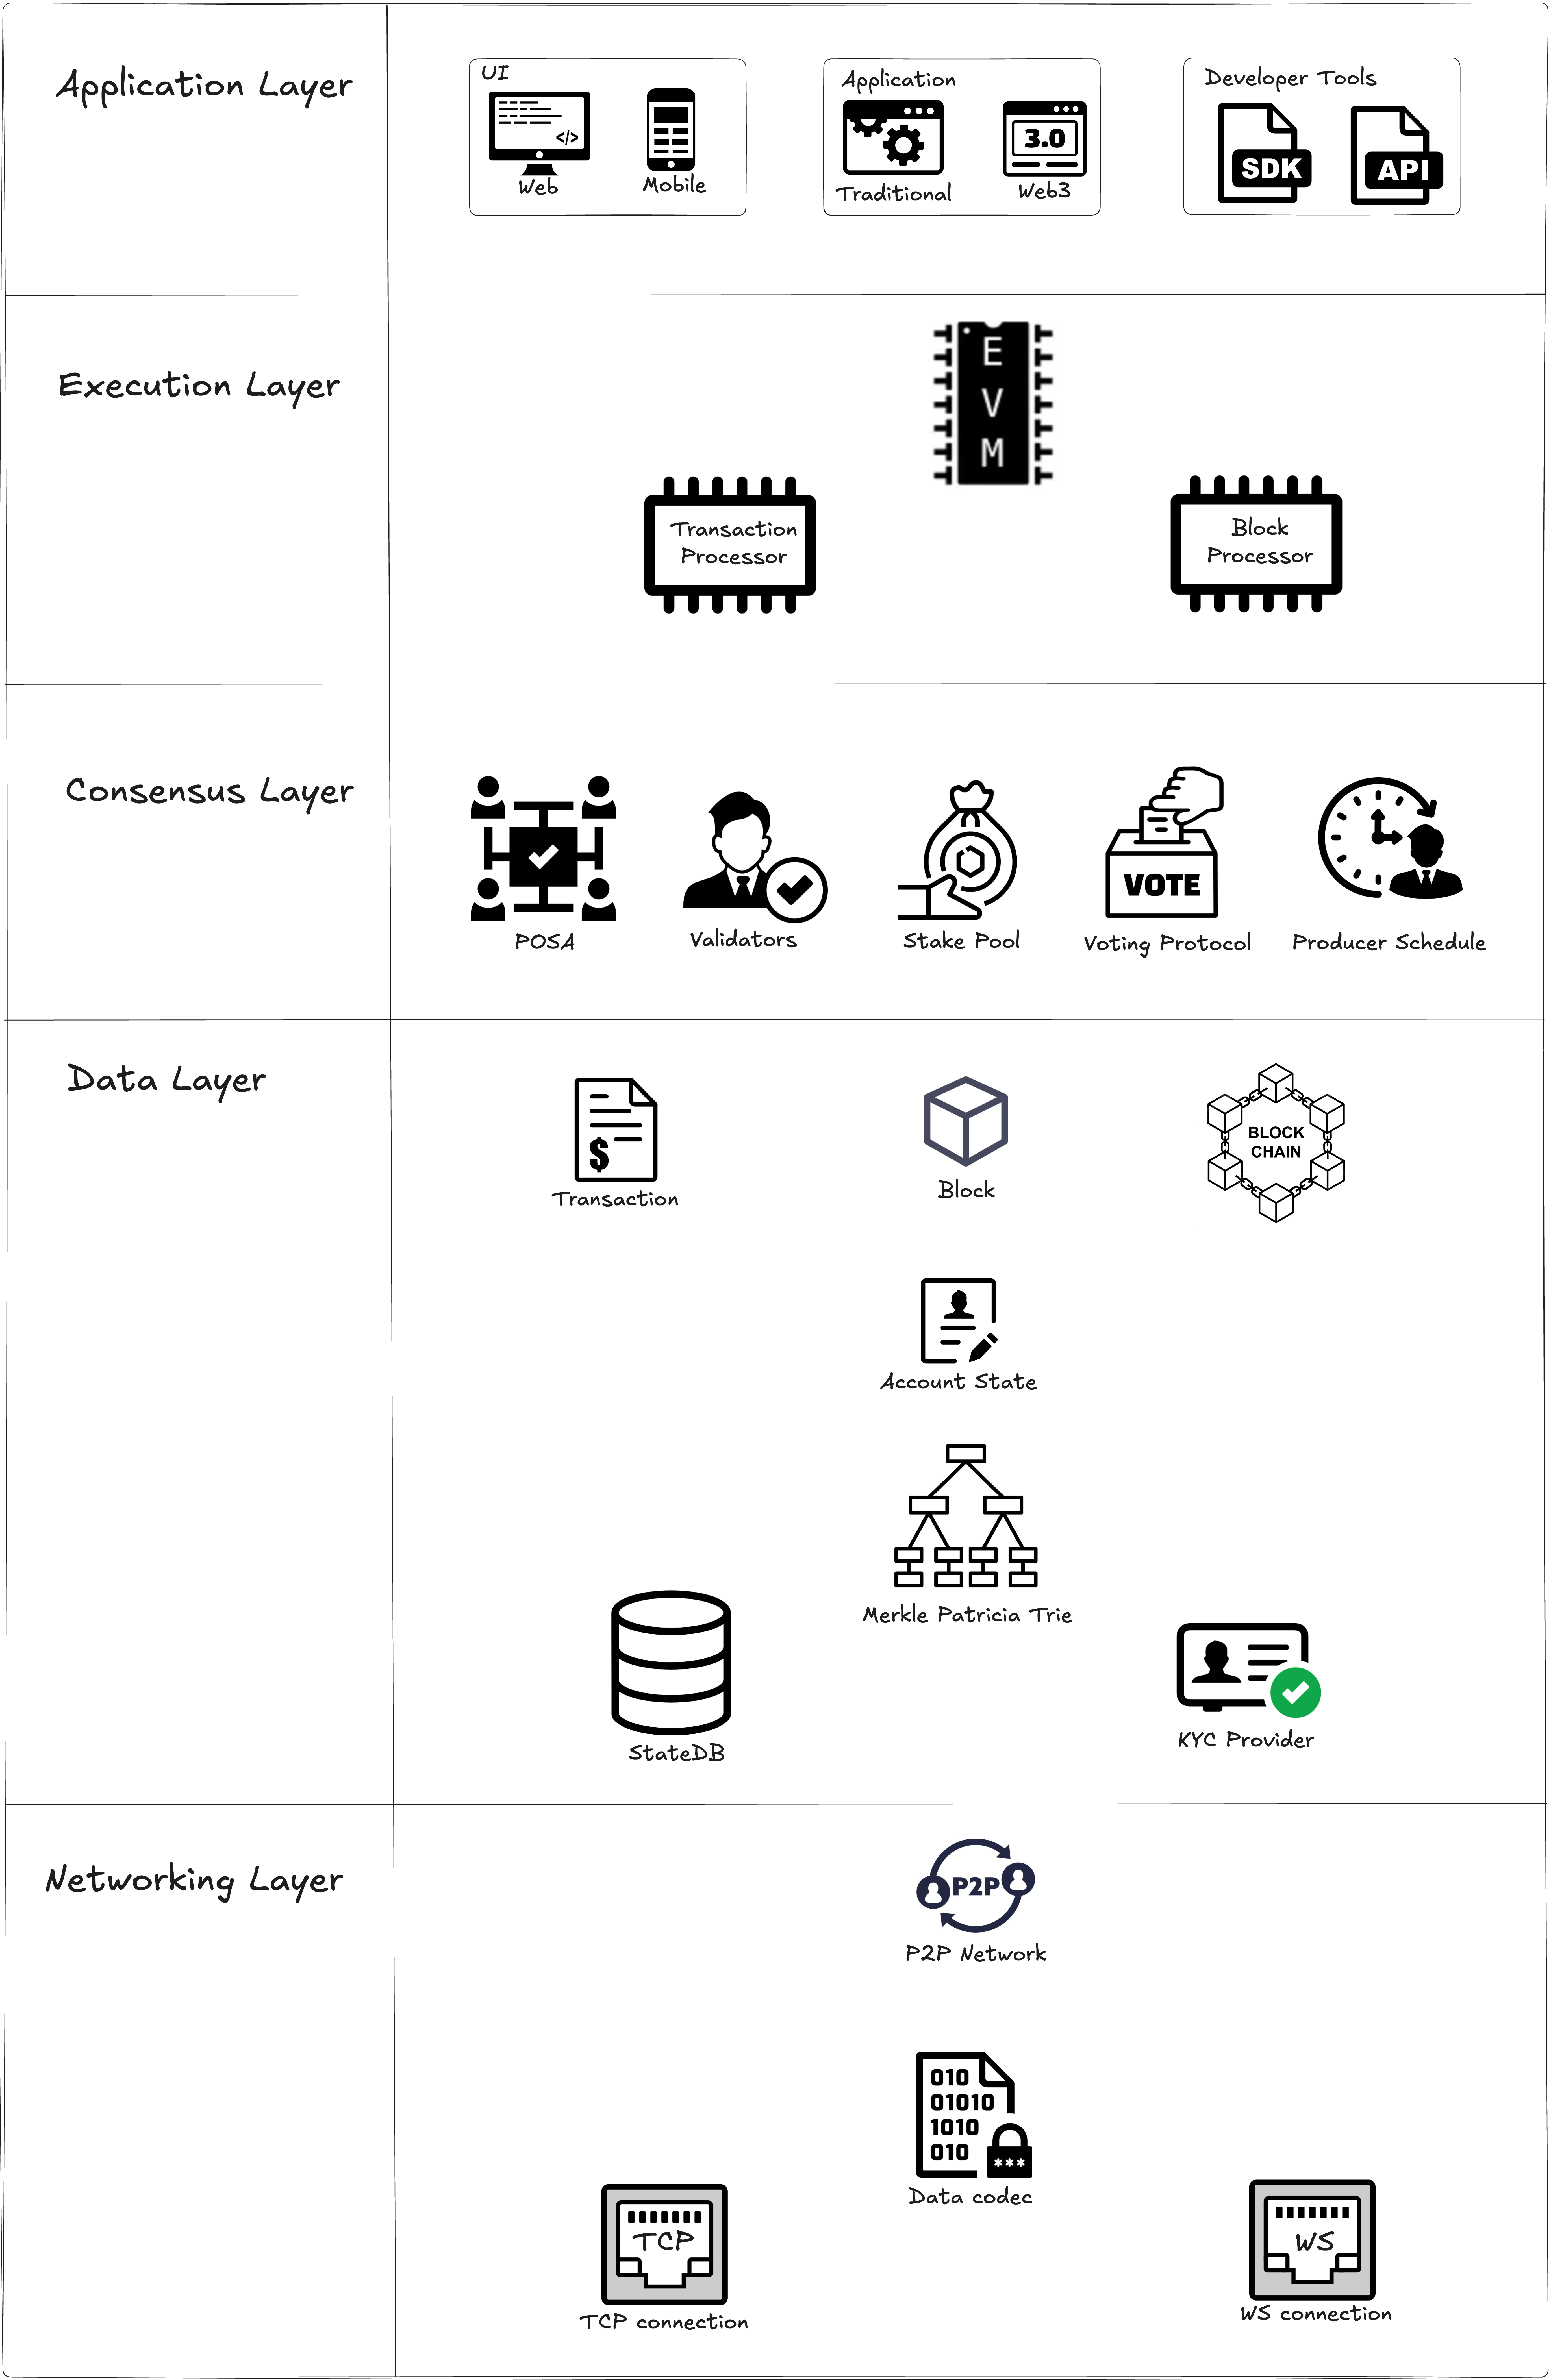
\includegraphics[width=0.9\textwidth]{architecture.png} 
    \caption{Sơ đồ kiến trúc các lớp của Fichain.}
    \label{fig:architecture}
\end{figure}

\begin{itemize}
    \item \textbf{Lớp Ứng dụng (Application Layer):} Đây là lớp giao tiếp trực tiếp với người dùng cuối và nhà phát triển. Nó bao gồm giao diện người dùng (UI) cho Web và Di động, các ứng dụng (Truyền thống và Web3), và các công cụ dành cho nhà phát triển như SDK và API để xây dựng và tích hợp các ứng dụng phi tập trung (DApps).

    \item \textbf{Lớp Thực thi (Execution Layer):} Chịu trách nhiệm xử lý logic của hệ thống. Lớp này chứa Máy ảo Ethereum (EVM) để thực thi các hợp đồng thông minh, cùng với Bộ xử lý Giao dịch (Transaction Processor) và Bộ xử lý Khối (Block Processor) để xử lý và xác thực các hoạt động trên chuỗi.

    \item \textbf{Lớp Đồng thuận (Consensus Layer):} Đảm bảo tính toàn vẹn và nhất quán của toàn mạng lưới. Fichain sử dụng cơ chế đồng thuận PoSA (Proof of Staked Authority), trong đó các Validators được chọn để tạo khối mới. Lớp này cũng bao gồm các thành phần như Bể khoá cọc(Stake Pool), Giao thức Bỏ phiếu (Voting Protocol) và Lịch trình sản xuất khối (Producer Schedule).

    \item \textbf{Lớp Dữ liệu (Data Layer):} Quản lý việc lưu trữ tất cả dữ liệu của chuỗi khối. Các thành phần chính bao gồm cấu trúc của Giao dịch (Transaction), Khối (Block) và toàn bộ Chuỗi khối (Blockchain). Lớp này cũng quản lý Trạng thái tài khoản (Account State), sử dụng cây Merkle Patricia Trie để đảm bảo tính toàn vẹn dữ liệu, lưu trữ trạng thái trong StateDB, và có thể tích hợp với Nhà cung cấp KYC.

    \item \textbf{Lớp Mạng (Networking Layer):} Quản lý việc giao tiếp giữa các nút (nodes) trong mạng lưới. Lớp này hoạt động trên một mạng ngang hàng (P2P Network), sử dụng các giao thức kết nối như TCP và WebSocket (WS), và một bộ mã hóa/giải mã dữ liệu (Data codec) để truyền thông tin một cách an toàn và hiệu quả.
\end{itemize}

\section{Giá trị thực tiễn}
Fichain mở ra các mô hình kinh doanh mới, tối ưu hóa hoạt động hiện tại và tạo nền tảng cho các hệ sinh thái Web3 trong lĩnh vực tài chính - ngân hàng và kinh tế số.

\subsection{Đối với Ngân hàng và Tổ chức Tài chính}
\begin{itemize}
    \item \textbf{Số hóa Tài sản \& Chứng khoán (Asset Tokenization):} Cho phép phát hành, quản lý và giao dịch các loại tài sản được mã hóa như trái phiếu doanh nghiệp, chứng chỉ quỹ, bất động sản một cách minh bạch, hiệu quả và giảm thiểu chi phí phát hành.
    \item \textbf{Thanh toán Xuyên biên giới:} Xây dựng hệ thống chuyển tiền và thanh toán quốc tế tức thì, chi phí thấp, giảm sự phụ thuộc vào các mạng lưới trung gian truyền thống (như SWIFT\cite{swift_website}, VISA\cite{visa_website}) và tăng tốc độ thanh khoản.
    \item \textbf{Tài chính Doanh nghiệp \& Tín dụng:} Tạo lập các nền tảng cho vay ngang hàng (P2P Lending), tài trợ thương mại (Trade Finance), quản lý chuỗi cung ứng trên blockchain, tăng cường tính minh bạch và hiệu quả trong việc thẩm định và giải ngân.
    \item \textbf{Hiện đại hóa Core Banking \& Liên kết Web3:} Giảm tải cho các hệ thống core banking kế thừa bằng cách chuyển các nghiệp vụ mới lên một nền tảng linh hoạt, bảo mật và dễ tích hợp với các dịch vụ Web3, smart contract và các ứng dụng phi tập trung (DApp), đồng thời mở ra khả năng tương tác với các hệ thống ngân hàng kỹ thuật số trong và ngoài nước.
\end{itemize}

\subsection{Đối với Nền kinh tế và Xã hội}
\begin{itemize}
    \item \textbf{Thúc đẩy tài chính toàn diện:} Giảm chi phí giao dịch và tạo ra các sản phẩm tài chính mới, dễ tiếp cận hơn cho người dân và doanh nghiệp nhỏ.
    \item \textbf{Nâng cao năng lực công nghệ quốc gia:} Việc làm chủ một công nghệ nền tảng như blockchain Layer 1 không chỉ khẳng định vị thế công nghệ của Việt Nam, mà còn cho phép tích hợp sâu với các dịch vụ công của chính phủ như định danh số (eKYC), quản lý tài sản công, lưu trữ hồ sơ y tế và giáo dục, góp phần xây dựng chính phủ số hiệu quả và minh bạch.
\end{itemize}

\section{Tính sáng tạo}
Fichain khác biệt so với các giải pháp hiện có nhờ vào sự kết hợp của các yếu tố độc đáo, được thiết kế chuyên biệt.

\begin{itemize}
  \item \textbf{Lựa chọn Native Coin thực tiễn, không đầu cơ:} Trong khi hầu hết các blockchain Layer 1 tạo ra một native coin mới với giá trị biến động và mang tính đầu cơ (như ETH\cite{buterin2014ethereum}, SOL\cite{yakovenko2017solana}, AVAX\cite{rocket2019scalable}, ATOM\cite{kwon2016cosmos}), Fichain có một lựa chọn thiết kế mang tính đột phá và thực tiễn: \textbf{sử dụng Việt Nam Đồng làm đơn vị tiền tệ gốc}. Cách tiếp cận này loại bỏ rào cản về tâm lý và rủi ro biến động giá, trực tiếp giải quyết mối quan tâm hàng đầu của các tổ chức tài chính và cơ quan quản lý.

  \begin{itemize}
        \item Cơ chế đồng thuận \textbf{PoSA} yêu cầu các validator phải là những định chế tài chính được cấp phép và có định danh (Authority), đảm bảo chỉ những bên đáng tin cậy mới có quyền tham gia xác thực giao dịch.
        \item Nền tảng cho phép thiết lập các \textbf{mạng riêng tư (private) hoặc liên minh (consortium)}, toàn quyền kiểm soát việc truy cập và chia sẻ dữ liệu.
        \item Khả năng tích hợp sẵn các quy trình \textbf{KYC/AML} ở cấp độ giao thức, đảm bảo mọi giao dịch đều có thể truy vết và tuân thủ pháp luật.
  \end{itemize}
    

    \item \textbf{Hạ tầng tương thích Web2 và mở rộng sang Web3:} Fichain được thiết kế để có thể tích hợp dễ dàng với các hệ thống tài chính truyền thống thông qua API chuẩn hóa, đồng thời mở ra khả năng kết nối với các ứng dụng Web3 hiện đại. Điều này giúp các ngân hàng và tổ chức tài chính từng bước chuyển đổi mà không bị gián đoạn, tận dụng cả hạ tầng hiện tại và tiềm năng phi tập trung trong tương lai.

    \item \textbf{Khả năng tích hợp dịch vụ công và định danh số:} Không chỉ phục vụ khối ngân hàng, Fichain còn hướng tới khả năng tích hợp với các dịch vụ công như định danh điện tử (eKYC), quản lý hồ sơ thuế, hồ sơ công dân, và các dịch vụ hành chính số. Điều này mang lại một kiến trúc blockchain linh hoạt, có thể phục vụ cả khối tư nhân lẫn nhà nước trong hệ sinh thái tài chính số toàn diện.

  \item \textbf{Kiến trúc Cầu nối An toàn giữa Tài chính Truyền thống và Tương lai Số:}
    Fichain không đặt mục tiêu thay thế hoàn toàn hệ thống core banking, mà định vị mình là một "cầu nối" chiến lược và an toàn. Nền tảng cho phép các ngân hàng giữ nguyên hệ thống lõi ổn định của mình, đồng thời sử dụng Fichain như một "sandbox" đổi mới để:
    \begin{itemize}
        \item \textbf{Thử nghiệm và triển khai} các sản phẩm tài chính số (số hóa tài sản, DeFi) một cách nhanh chóng và ít rủi ro.
        \item \textbf{Kết nối} một cách an toàn giữa dữ liệu trong hệ thống kế thừa và các ứng dụng trên blockchain.
        \item \textbf{Từng bước hiện đại hóa} các dịch vụ mà không gây gián đoạn cho hoạt động kinh doanh cốt lõi. Đây là một lộ trình chuyển đổi số thực tế và khả thi cho các tổ chức tài chính lớn.
    \end{itemize}

\end{itemize}

\section{Tính khả thi và khả năng mở rộng}

\subsection{Tính khả thi kỹ thuật}
Tính khả thi kỹ thuật của Fichain được đảm bảo bởi năng lực và kinh nghiệm của đội ngũ phát triển. Đội ngũ bao gồm các chuyên gia hàng đầu về:
\begin{itemize}
    \item \textbf{Phát triển Blockchain Layer 1:} Có kinh nghiệm thiết kế, xây dựng, tối ưu và vận hành mainnet cho blockchain Layer 1 với hiệu suất cao (hàng nghìn TPS).
    \item \textbf{Phát triển DApps và Smart Contract:} Am hiểu sâu sắc về EVM, Solidity, và các tiêu chuẩn token phổ biến.
    \item \textbf{Core Banking và Tích hợp hệ thống:} Có kinh nghiệm thực tế trong việc tích hợp các hệ thống ngân hàng lõi với các hệ thống vệ tinh, tuân thủ các giao thức và quy định của ngành.
    \item \textbf{Khoa học dữ liệu và AI trong tài chính:} Có khả năng xây dựng các mô hình AI/ML cho các bài toán như đánh giá rủi ro, phát hiện gian lận.
\end{itemize}
Sự kết hợp này khẳng định đội ngũ có đủ năng lực để xây dựng, triển khai và hỗ trợ vận hành Fichain.

\subsection{Tính khả thi tài chính và mô hình kinh doanh}
Fichain lựa chọn mô hình kinh doanh B2B với định hướng hợp tác linh hoạt và đa dạng, phù hợp với nhiều loại hình doanh nghiệp. Các hình thức hợp tác bao gồm:
\begin{itemize}
    \item \textbf{Phí giấy phép sử dụng nền tảng (Licensing Fee)}: Áp dụng cho các đối tác có nhu cầu tích hợp và triển khai nền tảng Fichain vào hệ thống riêng.
    \item \textbf{Phí giao dịch (Transaction Fee)}: Thu phí trên mỗi giao dịch được thực hiện qua nền tảng.
    \item \textbf{Mô hình chia sẻ doanh thu (Revenue Sharing)}: Thỏa thuận chia sẻ lợi nhuận linh hoạt, dựa trên quy mô và đặc thù của từng dự án hợp tác.
\end{itemize}
Cấu trúc doanh thu này giúp Fichain đảm bảo tính ổn định và bền vững về tài chính, đồng thời tạo điều kiện thuận lợi để mở rộng hệ sinh thái và đầu tư vào phát triển công nghệ lâu dài.

\subsection{Tính khả thi pháp lý}
Fichain được thiết kế với sự tuân thủ pháp lý là cốt lõi. Nền tảng cho phép:
\begin{itemize}
    \item Triển khai dưới dạng mạng riêng tư (private) hoặc liên minh (consortium), cho phép kiểm soát hoàn toàn danh tính các bên tham gia.
    \item Tích hợp các quy trình KYC/AML.
    \item Phân quyền truy cập dữ liệu giao dịch, đáp ứng yêu cầu của cơ quan quản lý khi cần thiết.
\end{itemize}

\subsection{Khả năng mở rộng (Scalability)}
Nền tảng Fichain được thiết kế để có khả năng mở rộng cao ngay từ đầu, với mục tiêu xử lý hàng nghìn giao dịch mỗi giây (TPS) nhờ cơ chế đồng thuận PoSA hiệu quả. Kiến trúc này đủ sức đáp ứng nhu cầu giao dịch của các ứng dụng tài chính quy mô lớn.

\section{Lộ trình Phát triển Chi tiết (Roadmap)}

\begin{itemize}
    \item \textbf{Giai đoạn 1 (Q2 2025): Nền tảng \& Thử nghiệm Nội bộ}
    \begin{itemize}
        \item Hoàn thiện MVP (Web/Desktop) và ra mắt bản thử nghiệm Alpha.
        \item Khởi động R\&D cho Ứng dụng Di động và Thiết bị Ví cứng.
        \item Xây dựng bộ nhận diện thương hiệu và các kênh truyền thông ban đầu.
    \end{itemize}

    \item \textbf{Giai đoạn 2 (Q3 2025): Thử nghiệm Mở rộng \& Thu thập Phản hồi}
    \begin{itemize}
        \item Ra mắt bản Beta công khai, thu thập phản hồi để cải thiện UX/UI.
        \item Bắt đầu phát triển chính thức Ứng dụng Di động (iOS \& Android).
        \item Hoàn thiện và thử nghiệm nguyên mẫu (prototype) Ví cứng.
    \end{itemize}

    \item \textbf{Giai đoạn 3 (Q4 2025): Ra mắt Chính thức \& Tích hợp}
    \begin{itemize}
        \item Ra mắt chính thức phiên bản 1.0 (Web/Desktop).
        \item \textbf{Tích hợp Ngân hàng:} Triển khai tính năng Mua/Bán tài sản số (On-ramp/Off-ramp) qua cổng thanh toán.
        \item Phát hành bản Beta cho Ứng dụng Di động.
        \item Triển khai chiến dịch marketing quy mô lớn.
    \end{itemize}

    \item \textbf{Giai đoạn 4 (2026+): Mở rộng Hệ sinh thái Toàn diện}
    \begin{itemize}
        \item \textbf{Hoàn thiện sản phẩm:} Ra mắt chính thức Ứng dụng Di động và mở bán Thiết bị Ví cứng chuyên biệt.
        \item \textbf{Tài chính Nâng cao:} Phát hành thẻ thanh toán vật lý/ảo, tích hợp sâu các dịch vụ DeFi (Staking, Lending).
        \item \textbf{Phát triển nền tảng:} Xây dựng API/SDK cho đối tác, ra mắt Launchpad, mở rộng thị trường quốc tế.
    \end{itemize}
\end{itemize}

\section{Đội ngũ}
Sức mạnh của Fichain đến từ sự kết hợp giữa kinh nghiệm chuyên sâu về blockchain Layer 1, Core Banking và Khoa học dữ liệu của đội ngũ chuyên gia Việt Nam.

\begin{itemize}
    \item \textbf{Hiếu Phan - Trưởng nhóm (Phát triển Layer 1):} 
    Chuyên sâu về thiết kế, xây dựng và tối ưu core blockchain engine (transaction pool, consensus, P2P, state machine), EVM. Có kinh nghiệm triển khai nhiều cơ chế đồng thuận (PoW, PoS, DPoS, PoA), tối ưu hiệu suất cao (hàng nghìn TPS), và vận hành mainnet Layer 1.

    \item \textbf{Hân Phạm - Lập trình viên Layer 1 \& DevOps:} 
    Phát triển và bảo trì các thành phần cốt lõi blockchain, thiết lập CI/CD, phát triển smart contract (Solidity) và DApp frontend. Nghiên cứu Layer 2 và cross-chain.

    \item \textbf{Nguy Nguyễn - Lập trình viên DApps:} 
    Chuyên sâu thiết kế, phát triển smart contract (Solidity, Hardhat, tối ưu gas, bảo mật). Phát triển frontend DApp và backend. Kinh nghiệm với GameFi, DeFi (DEX, Bridge), và xử lý dữ liệu on-chain.

    \item \textbf{Hải Trần - Lập trình viên Core Banking:} 
    Có kinh nghiệm tích hợp hệ thống core banking quy mô lớn với các hệ thống vệ tinh (eKYC, ví điện tử), thành thạo các giao thức tích hợp (SOAP, REST, ISO 8583) và tuân thủ quy định NHNN.

    \item \textbf{Hùng Hà - Chuyên viên Phân tích Dữ liệu Ngân hàng:} 
    Có kinh nghiệm tích hợp hệ thống core banking, vận hành CSDL lớn. Xây dựng và triển khai pipeline AI/ML (Python, TensorFlow/PyTorch) cho các bài toán tài chính (phân loại rủi ro, phát hiện gian lận, scoring tín dụng).

\end{itemize}

\section{Các khó khăn và bài học kinh nghiệm}
Trong quá trình nghiên cứu và phát triển Fichain, đội ngũ đã đối mặt với nhiều thách thức đặc thù, từ đó rút ra những bài học kinh nghiệm quý báu định hình nên kiến trúc và chiến lược của dự án.

\subsection{Khó khăn đã gặp}
\begin{itemize}

     \item \textbf{Làm chủ và Xây dựng Công nghệ Lõi Blockchain từ Con số Không:}
       Để đạt được sự tùy biến và tối ưu tuyệt đối cho ngành tài chính, đội ngũ đã lựa chọn không sử dụng các framework blockchain có sẵn (như Cosmos SDK\cite{kwon2016cosmos} hay Substrate\cite{substrate_docs}) mà tự xây dựng nền tảng từ các thành phần cơ bản. Điều này đặt ra một khối lượng công việc khổng lồ và thách thức kỹ thuật nền tảng:
    \begin{itemize}
        \item \textbf{Tích hợp sâu Ethereum Virtual Machine (EVM):} Đây không chỉ là việc "nhúng" EVM, mà là một quá trình phức tạp để kết nối máy ảo với lớp quản lý trạng thái (state management) của Fichain, đảm bảo việc đọc/ghi trạng thái và xử lý `gas` diễn ra chính xác, hiệu quả và tương thích với các công cụ phát triển của hệ sinh thái Ethereum.
        \item \textbf{Phát triển lớp mạng P2P (Peer-to-Peer):} Phải tự thiết kế và triển khai toàn bộ giao thức mạng, bao gồm cơ chế khám phá node (node discovery), lan truyền giao dịch và khối (gossip protocol), và đồng bộ hóa chuỗi (chain synchronization) một cách an toàn và tối ưu.
    \end{itemize}

    \item \textbf{Cân bằng giữa Hiệu suất, Bảo mật và Tuân thủ trong cơ chế PoSA:}
    Việc thiết kế cơ chế đồng thuận PoSA là một bài toán cân bằng tinh vi.
    \begin{itemize}
        \item Nếu quá chú trọng vào hiệu suất (bằng cách giảm số lượng validator), hệ thống có thể trở nên quá tập trung và kém an toàn.
        \item Ngược lại, nếu yêu cầu về stake (ký quỹ) quá cao để tăng cường an ninh, sẽ tạo ra rào cản lớn cho các tổ chức tài chính nhỏ hơn muốn tham gia mạng lưới.
        \item Việc tích hợp các yếu tố "Authority" (định danh) vào thuật toán đòi hỏi phải giải quyết vấn đề quản trị: Ai có quyền cấp và thu hồi "Authority"? Quy trình này diễn ra như thế nào để đảm bảo tính công bằng?
    \end{itemize}

    \item \textbf{Tích hợp với hệ thống Core Banking kế thừa:}
    Việc kết nối một hệ thống phân tán, bất biến (blockchain) với một hệ thống tập trung, có thể chỉnh sửa (core banking) là một thách thức lớn về kỹ thuật. Các vấn đề chính bao gồm độ trễ dữ liệu, đảm bảo tính nhất quán (consistency) giữa hai hệ thống, và thiết kế các giao thức giao tiếp (API/Adapter) an toàn, hiệu quả.
\end{itemize}

\subsection{Bài học kinh nghiệm}
\begin{itemize}
    \item \textbf{Công nghệ phải đi đôi với quy trình vận hành:}
    Bài học lớn nhất từ việc thiết kế native coin dựa trên VND là một giải pháp blockchain cho ngành tài chính không thể chỉ tồn tại trên phương diện công nghệ. Thành công của nó phụ thuộc rất lớn vào việc xây dựng một \textbf{khung pháp lý và quy trình vận hành (operational framework)} chặt chẽ giữa thế giới on-chain và off-chain. Cần có sự tham gia của các bên thứ ba như đơn vị kiểm toán, ngân hàng lưu ký để đảm bảo tính minh bạch và tin cậy.

    \item \textbf{Tầm quan trọng của việc mô phỏng và kiểm thử thực tế (Simulation \& Real-world Testing):}
    Đối với cơ chế đồng thuận, không có lý thuyết nào là hoàn hảo. Đội ngũ đã học được rằng cách tốt nhất để tinh chỉnh các tham số (số lượng validator, mức stake tối thiểu, cơ chế phạt...) là thông qua việc \textbf{xây dựng các môi trường mô phỏng} các kịch bản tấn công và chạy thử nghiệm trong một mạng testnet có điều kiện gần giống với thực tế nhất.

    \item \textbf{Xây dựng "Lớp Chuyển đổi" thay vì cố gắng "Thay thế":}
    Thay vì cố gắng thay thế hoàn toàn hệ thống cũ, bài học kinh nghiệm là nên tập trung vào việc \textbf{xây dựng các "lớp chuyển đổi" (Adapter Layers) thông minh}. Các lớp này đóng vai trò là cầu nối, xử lý việc phiên dịch, đệm dữ liệu và đồng bộ hóa giữa Fichain và các hệ thống core banking. Cách tiếp cận này giúp giảm thiểu rủi ro, cho phép triển khai từng phần và mang lại giá trị nhanh hơn cho đối tác.

    \item \textbf{Tập trung là sức mạnh:}
    Trong một thế giới blockchain đầy rẫy các dự án "làm tất cả mọi thứ", bài học cốt lõi là việc \textbf{tập trung giải quyết một bài toán cụ thể cho một ngành dọc cụ thể} (tài chính - ngân hàng) là con đường hiệu quả nhất. Sự tập trung này cho phép đưa ra những quyết định thiết kế táo bạo và phù hợp (như dùng VND làm native coin), điều mà các nền tảng đa năng không thể làm được.
\end{itemize}


\newpage % Ngắt trang trước khi tới phần tài liệu tham khảo

% --- TÀI LIỆU THAM KHẢO ---
\section{Tài liệu tham khảo}
\bibliographystyle{plain} % Kiểu trình bày danh mục tham khảo
\bibliography{references} % Gọi tệp references.bib

\end{document}
